\section{\textbf{Results}}
We analyze the speedupss obtained by the proposed Parallel Automata Processor Architecture (PAP).
\subsection{Overall Speedup}
Figure 5 shows the speedups obtained by the propose we are analyzing, Parallel
Automata Processor Architecture (PAP), when compared to the
baseline AP architecture. We present speedups for both 1 AP rank
(8 D480 devices) and 4 AP ranks (32 D480 devices in the current
AP generation) and 1 MB and 10 MB input streams. We also exploit
the parallelism offered by each of the half-cores in a D480 device
when our FSMs can fit in a single half-core. 
\begin{figure}[t]
    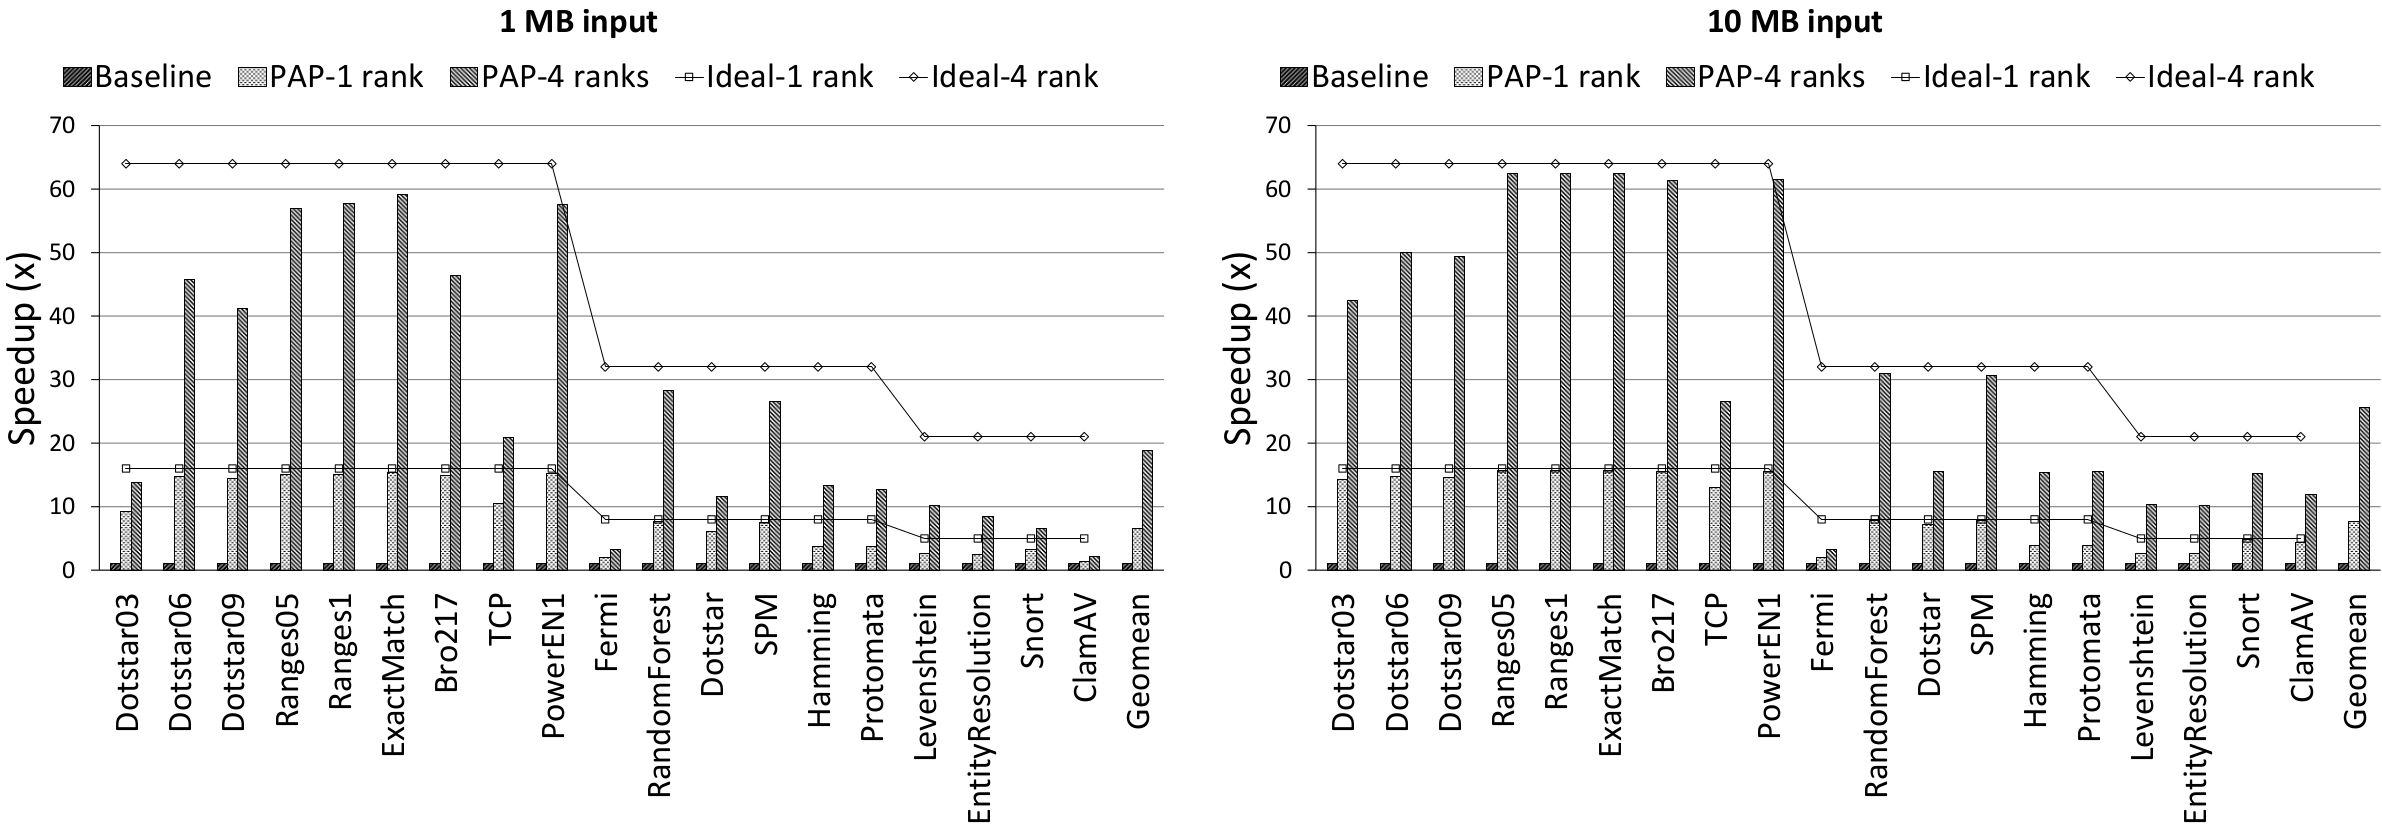
\includegraphics[width=\textwidth]{f4.png}
    \centering
    \caption{Speedups obtained by the proposed architecture Parallel Automata Processor Architecture}
\end{figure}

It can be seen from the figure that PAP outperforms the sequential
AP baseline for most benchmarks. A noticeable trend is the larger
performance gains with the 10 MB stream. This is because the larger stream provides opportunity for creating larger input segments.
These larger input segments help in reducing in the number of active
flows due to the deactivation and convergence properties of the
FSMs  and the associated flow
switching overhead. Furthermore, large input segments also help
amortize the cost of false path invalidation and input composition
in the CPU.

\subsection{Overheads}

\subsubsection{Flow Switching}
It can be seen from Figure 6  that the overheads of context switching between flows are
less than 2\% for most benchmarks. As discussed before, since the
number of active flows greatly reduces as input symbols are processed, the corresponding convergence and deactivation checking
overheads also reduce.
\begin{figure}[!]
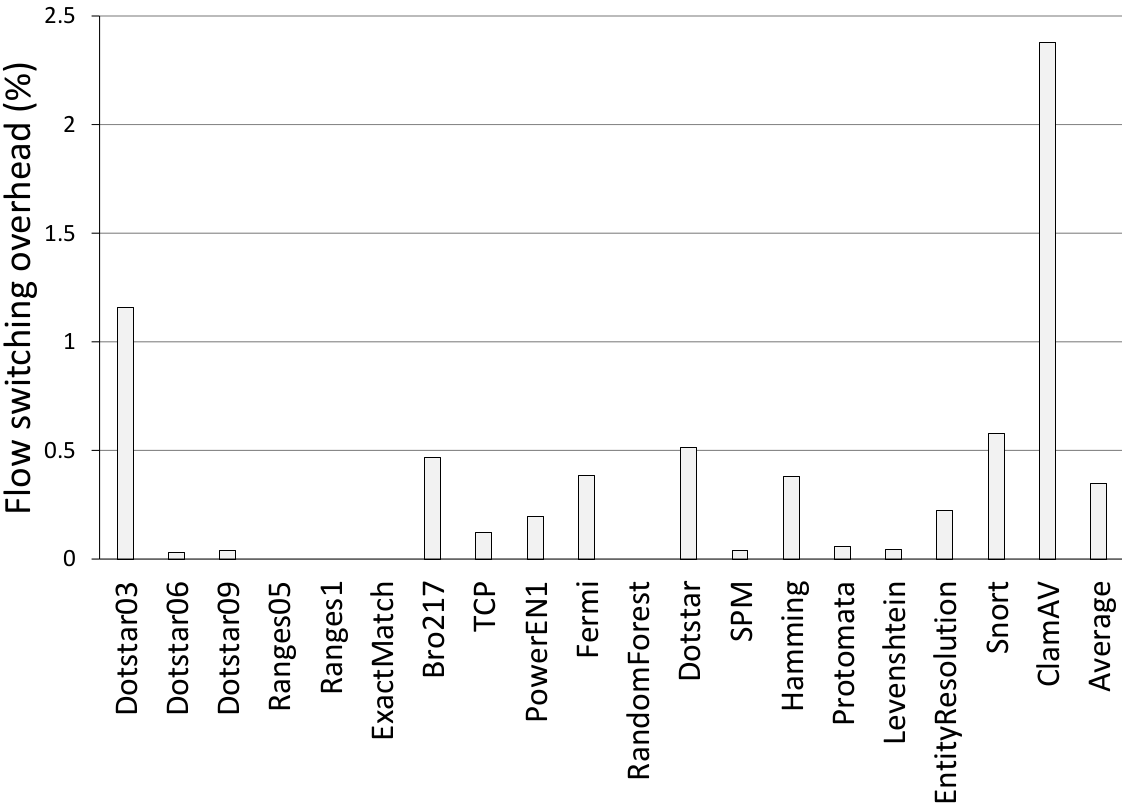
\includegraphics[width=0.5\textwidth]{f5.png}
\centering
\caption{Costs of flow switching.}
\end{figure}

\subsubsection{False Path Decoding} 
Figure 7 illustrates the overheads of decoding false paths at the host CPU after an input segment finishes
and sending a flow invalidation vector (FIV) to the next segment.
On an average most benchmarks see around 2000 symbol cycles
overhead. Fortunately, this cost is largely amortized because of two
reasons: (1) it can be overlapped with symbol processing in subsequent segments, (2) these invalidations are infrequent since several
flows have either already converged or have been deactivated and do
not require this invalidation.
\begin{figure}[!]
    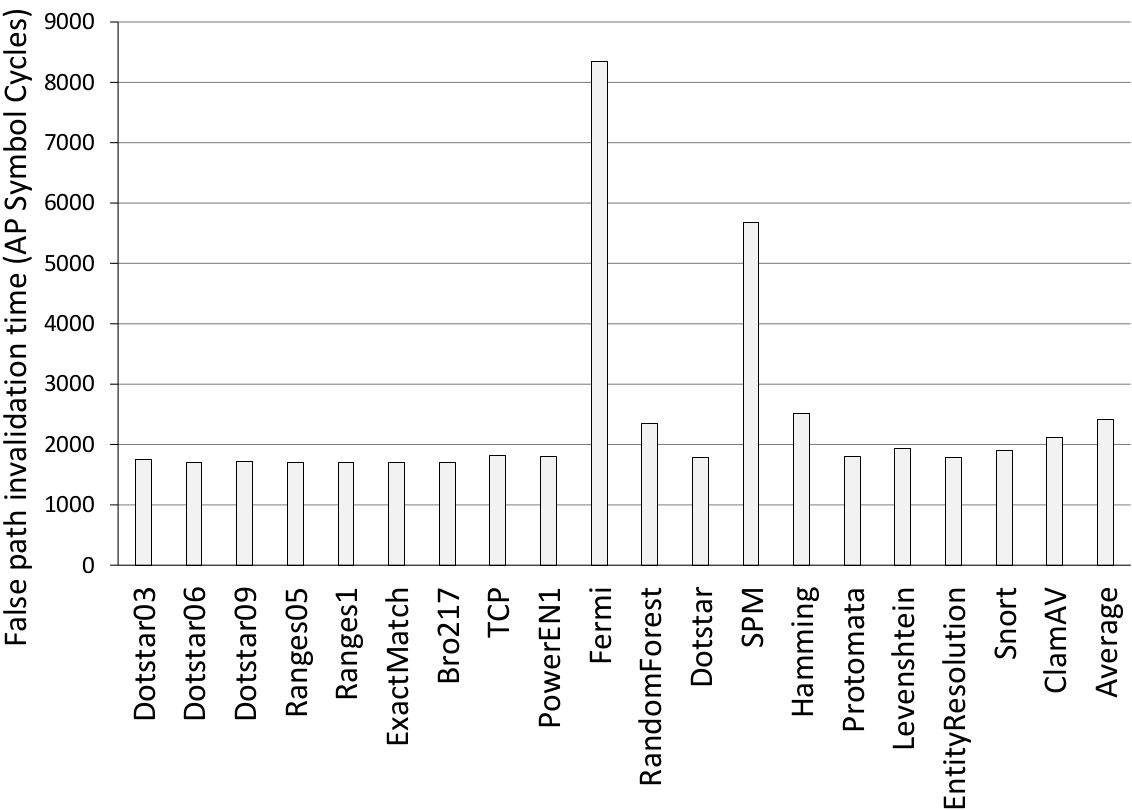
\includegraphics[width=0.5\textwidth]{f6.png}
    \centering
    \caption{Costs of decoding false paths at the end of input seg-
    ment.}
\end{figure}